%% LyX 2.2.3 created this file.  For more info, see http://www.lyx.org/.
%% Do not edit unless you really know what you are doing.
\documentclass[12pt,english]{article}
\usepackage[osf]{mathpazo}
\renewcommand{\sfdefault}{lmss}
\renewcommand{\ttdefault}{lmtt}
\usepackage[T1]{fontenc}
\usepackage[latin9]{inputenc}
\usepackage[paperwidth=30cm,paperheight=35cm]{geometry}
\geometry{verbose,tmargin=3cm,bmargin=3cm}
\setlength{\parindent}{0bp}
\usepackage{amsmath}
\usepackage{amssymb}

\makeatletter

%%%%%%%%%%%%%%%%%%%%%%%%%%%%%% LyX specific LaTeX commands.
%% Because html converters don't know tabularnewline
\providecommand{\tabularnewline}{\\}

%%%%%%%%%%%%%%%%%%%%%%%%%%%%%% User specified LaTeX commands.
\usepackage{tikz}
\usetikzlibrary{matrix,arrows,decorations.pathmorphing}
\usetikzlibrary{shapes.geometric}
\usepackage{tikz-cd}
\usepackage{amsthm}
\theoremstyle{plain}
\newtheorem{theorem}{Theorem}[section]
\newtheorem{lemma}[theorem]{Lemma}
\newtheorem{prop}{Proposition}[section]
\newtheorem*{cor}{Corollary}
\theoremstyle{definition}
\newtheorem{defn}{Definition}[section]
\newtheorem{ex}{Exercise} 
\newtheorem{example}{Example}[section]
\theoremstyle{remark}
\newtheorem*{rem}{Remark}
\newtheorem*{note}{Note}
\newtheorem{case}{Case}
\usepackage{graphicx}
\usepackage{amssymb}
\usepackage{tikz-cd}
\usetikzlibrary{calc,arrows,decorations.pathreplacing}
\tikzset{mydot/.style={circle,fill,inner sep=1.5pt},
commutative diagrams/.cd,
  arrow style=tikz,
  diagrams={>=latex},
}

\usepackage{babel}
\usepackage{hyperref}
\hypersetup{
    colorlinks,
    citecolor=black,
    filecolor=black,
    linkcolor=black,
    urlcolor=black
}
\usepackage{pgfplots}
\usetikzlibrary{decorations.markings}
\pgfplotsset{compat=1.9}

\makeatother

\usepackage{babel}
\begin{document}

\section*{Permutativity}

~~~We introduce a new type of algebraic law which we call the \textbf{permutative
law} since it corresponds with the permutohedron as the associative
law corresponds with associahedron.

\begin{defn} Let $A$ be a set equipped with a binary operation $\cdot:A\times A\to A$
and a unary operation $f:A\to A$. We say the triple $\mathcal{A}=(A,f,\cdot)$
is \textbf{permutative} when for all $a,b,c,d\in A$, 
\begin{equation}
(f(a)f(b))f(cd)=f(ab)(f(c)f(d))\label{eq:permutativelaw}
\end{equation}

\end{defn}

There's a very nice way of capturing this law in terms of Cayley ordered
Bell trees:

\begin{center}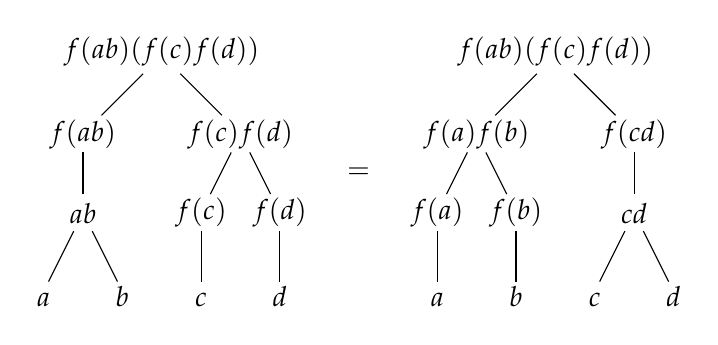
\begin{tikzpicture}

\node[label={[label distance=-0.45cm]90:$a$}] (a1) at (0,0) {};
\node[label={[label distance=-0.45cm]90:$b$}] (a2) at (1,0) {};
\node[label={[label distance=-0.45cm]90:$c$}] (a3) at (2,0) {};
\node[label={[label distance=-0.45cm]90:$d$}] (a4) at (3,0) {};

\node[label={[label distance=-0.5cm]90:$ab$}, inner sep=6.5pt] (b1) at (0.5,1) {};
\node[label={[label distance=-0.55cm]90:$f(c)$}, inner sep=6.5pt] (b2) at (2,1) {};
\node[label={[label distance=-0.55cm]90:$f(d)$}, inner sep=6.5pt] (b3) at (3,1) {};

\node[label={[label distance=-0.55cm]90:$f(ab)$}, inner sep=6.5pt] (c1) at (0.5,2) {};
\node[label={[label distance=-0.55cm]90:$f(c)f(d)$}, inner sep=6.5pt] (c2) at (2.5,2) {};

\node[label={[label distance=-0.5cm]90:$f(ab)(f(c)f(d))$}, inner sep=6.5pt] (d1) at (1.5,3) {};



\draw (a1) -- (b1);
\draw (a2) -- (b1);
\draw (a3) -- (b2);
\draw (a4) -- (b3);

\draw (b1) -- (c1);
\draw (b2) -- (c2);
\draw (b3) -- (c2);

\draw (c1) -- (d1);
\draw (c2) -- (d1);





\node[label={[label distance=-0.45cm]90:$a$}] (aa1) at (5,0) {};
\node[label={[label distance=-0.45cm]90:$b$}] (aa2) at (6,0) {};
\node[label={[label distance=-0.45cm]90:$c$}] (aa3) at (7,0) {};
\node[label={[label distance=-0.45cm]90:$d$}] (aa4) at (8,0) {};

\node[label={[label distance=-0.5cm]90:$cd$}, inner sep=6.5pt] (bb1) at (7.5,1) {};
\node[label={[label distance=-0.55cm]90:$f(a)$}, inner sep=6.5pt] (bb2) at (5,1) {};
\node[label={[label distance=-0.55cm]90:$f(b)$}, inner sep=6.5pt] (bb3) at (6,1) {};

\node[label={[label distance=-0.55cm]90:$f(cd)$}, inner sep=6.5pt] (cc1) at (7.5,2) {};
\node[label={[label distance=-0.55cm]90:$f(a)f(b)$}, inner sep=6.5pt] (cc2) at (5.5,2) {};

\node[label={[label distance=-0.5cm]90:$f(ab)(f(c)f(d))$}, inner sep=6.5pt] (dd1) at (6.5,3) {};



\draw (aa1) -- (bb2);
\draw (aa2) -- (bb3);
\draw (aa3) -- (bb1);
\draw (aa4) -- (bb1);

\draw (bb1) -- (cc1);
\draw (bb2) -- (cc2);
\draw (bb3) -- (cc2);

\draw (cc1) -- (dd1);
\draw (cc2) -- (dd1);

\node[] (x) at (4,1.5) {$=$};

\end{tikzpicture} \end{center}

This is analagous to how we can express the associative law in terms
of binary rooted trees:

\begin{center}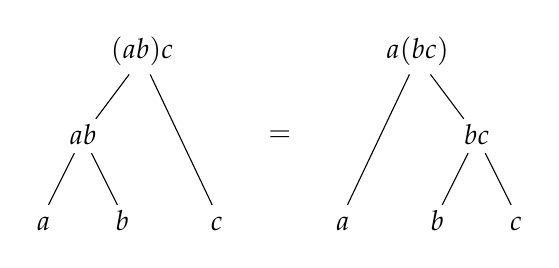
\begin{tikzpicture}

\node[label={[label distance=-0.45cm]90:$a$}] (a1) at (0,0) {};
\node[label={[label distance=-0.45cm]90:$b$}] (a2) at (1,0) {};
\node[label={[label distance=-0.45cm]90:$c$}] (a3) at (2.2,0) {};


\node[label={[label distance=-0.45cm]90:$ab$}, inner sep=6pt] (b1) at (0.5,1) {};

\node[label={[label distance=-0.45cm]90:$(ab)c$}, inner sep=6pt] (c1) at (1.25,2) {};


\draw (a1) -- (b1);
\draw (a2) -- (b1);

\draw (b1) -- (c1);
\draw (a3) -- (c1);


\node[label={[label distance=-0.45cm]90:$a$}] (aa1) at (3.8,0) {};
\node[label={[label distance=-0.45cm]90:$b$}] (aa2) at (5,0) {};
\node[label={[label distance=-0.45cm]90:$c$}] (aa3) at (6,0) {};

\node[label={[label distance=-0.45cm]90:$bc$}, inner sep=6pt] (bb2) at (5.5,1) {};

\node[label={[label distance=-0.45cm]90:$a(bc)$}, inner sep=6pt] (cc1) at (4.75,2) {};

\draw (aa2) -- (bb2);
\draw (aa3) -- (bb2);

\draw (aa1) -- (cc1);
\draw (bb2) -- (cc1);

\node[] (x) at (3,1) {$=$};

\end{tikzpicture} \end{center}

~~~The difference between these two types of trees is that the
Cayley ordered Bell trees keep track of a unary operator $f$, whereas
the binary rooted trees do not. The Cayley ordered Bell trees can
be attached to the vertices of the permutohedron and the ordered binary
rooted trees can be attached to the vertices of the associahedron.
There is a natural way to map the permutohedron to the associahedron,
and it correponds to forgetting the unary operator $f$. In the image
below, we draw the permutohedron $P_{2}$ as well as associahedron
$K_{2}$ inside of it. To each vertex of $K_{2}$, we can atach a
$4$-leaf ordered rooted binary tree. Also, to each vertex of $P_{2}$,
we can attach a $4$-leaf Cayley ordered Bell tree, which we do here.
The map from $P_{2}$ to $K_{2}$ is obtained by collapsing the red
edges. This can be interpreted as treating the unary operation $f$
as the identity function.

\begin{center}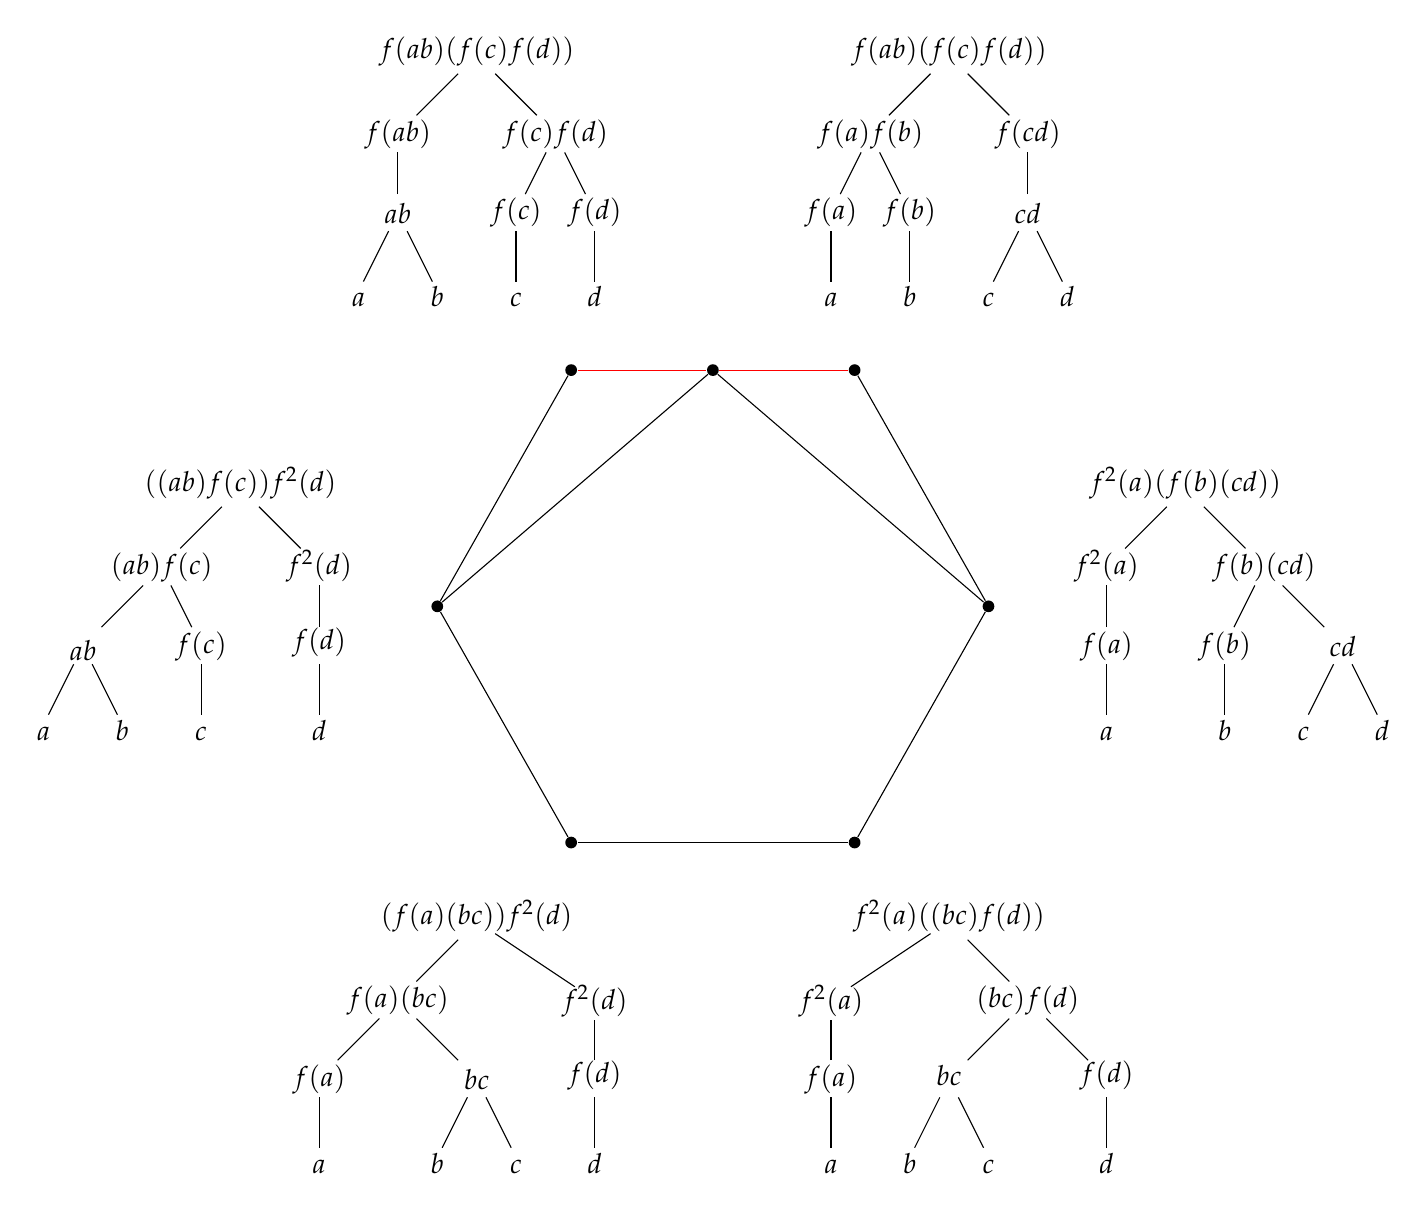
\begin{tikzpicture}
\node[label={[label distance=-0.45cm]90:$a$}] (a1) at (-0.5,0) {};
\node[label={[label distance=-0.45cm]90:$b$}] (a2) at (0.5,0) {};
\node[label={[label distance=-0.45cm]90:$c$}] (a3) at (1.5,0) {};
\node[label={[label distance=-0.45cm]90:$d$}] (a4) at (2.5,0) {};
\node[label={[label distance=-0.5cm]90:$ab$}, inner sep=6.5pt] (b1) at (0,1) {};
\node[label={[label distance=-0.55cm]90:$f(c)$}, inner sep=6.5pt] (b2) at (1.5,1) {};
\node[label={[label distance=-0.55cm]90:$f(d)$}, inner sep=6.5pt] (b3) at (2.5,1) {};
\node[label={[label distance=-0.55cm]90:$f(ab)$}, inner sep=6.5pt] (c1) at (0,2) {};
\node[label={[label distance=-0.55cm]90:$f(c)f(d)$}, inner sep=6.5pt] (c2) at (2,2) {};
\node[label={[label distance=-0.5cm]90:$f(ab)(f(c)f(d))$}, inner sep=6.5pt] (d1) at (1,3) {};
\draw (a1) -- (b1);
\draw (a2) -- (b1);
\draw (a3) -- (b2);
\draw (a4) -- (b3);
\draw (b1) -- (c1);
\draw (b2) -- (c2);
\draw (b3) -- (c2);
\draw (c1) -- (d1);
\draw (c2) -- (d1);

\node[label={[label distance=-0.45cm]90:$a$}] (aa1) at (5.5,0) {};
\node[label={[label distance=-0.45cm]90:$b$}] (aa2) at (6.5,0) {};
\node[label={[label distance=-0.45cm]90:$c$}] (aa3) at (7.5,0) {};
\node[label={[label distance=-0.45cm]90:$d$}] (aa4) at (8.5,0) {};
\node[label={[label distance=-0.5cm]90:$cd$}, inner sep=6.5pt] (bb1) at (8,1) {};
\node[label={[label distance=-0.55cm]90:$f(a)$}, inner sep=6.5pt] (bb2) at (5.5,1) {};
\node[label={[label distance=-0.55cm]90:$f(b)$}, inner sep=6.5pt] (bb3) at (6.5,1) {};
\node[label={[label distance=-0.55cm]90:$f(cd)$}, inner sep=6.5pt] (cc1) at (8,2) {};
\node[label={[label distance=-0.55cm]90:$f(a)f(b)$}, inner sep=6.5pt] (cc2) at (6,2) {};
\node[label={[label distance=-0.5cm]90:$f(ab)(f(c)f(d))$}, inner sep=6.5pt] (dd1) at (7,3) {};
\draw (aa1) -- (bb2);
\draw (aa2) -- (bb3);
\draw (aa3) -- (bb1);
\draw (aa4) -- (bb1);
\draw (bb1) -- (cc1);
\draw (bb2) -- (cc2);
\draw (bb3) -- (cc2);
\draw (cc1) -- (dd1);
\draw (cc2) -- (dd1);

\node[label={[label distance=-0.45cm]90:$a$}] (aaa1) at (9,-5.5) {};
\node[label={[label distance=-0.45cm]90:$b$}] (aaa2) at (10.5,-5.5) {};
\node[label={[label distance=-0.45cm]90:$c$}] (aaa3) at (11.5,-5.5) {};
\node[label={[label distance=-0.45cm]90:$d$}] (aaa4) at (12.5,-5.5) {};
\node[label={[label distance=-0.5cm]90:$cd$}, inner sep=6.5pt] (bbb1) at (12,-4.5) {};
\node[label={[label distance=-0.55cm]90:$f(a)$}, inner sep=6.5pt] (bbb2) at (9,-4.5) {};
\node[label={[label distance=-0.55cm]90:$f(b)$}, inner sep=6.5pt] (bbb3) at (10.5,-4.5) {};
\node[label={[label distance=-0.55cm]90:$f(b)(cd)$}, inner sep=6.5pt] (ccc1) at (11,-3.5) {};
\node[label={[label distance=-0.55cm]90:$f^2 (a)$}, inner sep=6.5pt] (ccc2) at (9,-3.5) {};
\node[label={[label distance=-0.5cm]90:$f^2 (a)(f(b)(cd))$}, inner sep=6.5pt] (ddd1) at (10,-2.5) {};
\draw (aaa1) -- (bbb2);
\draw (aaa2) -- (bbb3);
\draw (aaa3) -- (bbb1);
\draw (aaa4) -- (bbb1);
\draw (bbb1) -- (ccc1);
\draw (bbb2) -- (ccc2);
\draw (bbb3) -- (ccc1);
\draw (ccc1) -- (ddd1);
\draw (ccc2) -- (ddd1);

\node[label={[label distance=-0.45cm]90:$a$}] (aaaa1) at (5.5,-11) {};
\node[label={[label distance=-0.45cm]90:$b$}] (aaaa2) at (6.5,-11) {};
\node[label={[label distance=-0.45cm]90:$c$}] (aaaa3) at (7.5,-11) {};
\node[label={[label distance=-0.45cm]90:$d$}] (aaaa4) at (9,-11) {};
\node[label={[label distance=-0.5cm]90:$f(d)$}, inner sep=6.5pt] (bbbb1) at (9,-10) {};
\node[label={[label distance=-0.55cm]90:$f(a)$}, inner sep=6.5pt] (bbbb2) at (5.5,-10) {};
\node[label={[label distance=-0.45cm]90:$bc$}, inner sep=6.5pt] (bbbb3) at (7,-10) {};
\node[label={[label distance=-0.55cm]90:$(bc)f(d)$}, inner sep=6.5pt] (cccc1) at (8,-9) {};
\node[label={[label distance=-0.6cm]90:$f^2 (a)$}, inner sep=7pt] (cccc2) at (5.5,-9) {};
\node[label={[label distance=-0.5cm]90:$f^2 (a)((bc)f(d))$}, inner sep=6.5pt] (dddd1) at (7,-8) {};
\draw (aaaa1) -- (bbbb2);
\draw (aaaa2) -- (bbbb3);
\draw (aaaa3) -- (bbbb3);
\draw (aaaa4) -- (bbbb1);
\draw (bbbb1) -- (cccc1);
\draw (bbbb2) -- (cccc2);
\draw (bbbb3) -- (cccc1);
\draw (cccc1) -- (dddd1);
\draw (cccc2) -- (dddd1);

\node[label={[label distance=-0.45cm]90:$a$}] (aaaaa1) at (-1,-11) {};
\node[label={[label distance=-0.45cm]90:$b$}] (aaaaa2) at (0.5,-11) {};
\node[label={[label distance=-0.45cm]90:$c$}] (aaaaa3) at (1.5,-11) {};
\node[label={[label distance=-0.45cm]90:$d$}] (aaaaa4) at (2.5,-11) {};
\node[label={[label distance=-0.5cm]90:$f(d)$}, inner sep=6.5pt] (bbbbb1) at (2.5,-10) {};
\node[label={[label distance=-0.55cm]90:$f(a)$}, inner sep=6.5pt] (bbbbb2) at (-1,-10) {};
\node[label={[label distance=-0.5cm]90:$bc$}, inner sep=6.5pt] (bbbbb3) at (1,-10) {};
\node[label={[label distance=-0.6cm]90:$f^2 (d)$}, inner sep=7pt] (ccccc1) at (2.5,-9) {};
\node[label={[label distance=-0.55cm]90:$f(a)(bc)$}, inner sep=6.5pt] (ccccc2) at (0,-9) {};
\node[label={[label distance=-0.5cm]90:$(f(a)(bc))f^2 (d)$}, inner sep=6.5pt] (ddddd1) at (1,-8) {};
\draw (aaaaa1) -- (bbbbb2);
\draw (aaaaa2) -- (bbbbb3);
\draw (aaaaa3) -- (bbbbb3);
\draw (aaaaa4) -- (bbbbb1);
\draw (bbbbb1) -- (ccccc1);
\draw (bbbbb2) -- (ccccc2);
\draw (bbbbb3) -- (ccccc2);
\draw (ccccc1) -- (ddddd1);
\draw (ccccc2) -- (ddddd1);

\node[label={[label distance=-0.45cm]90:$a$}] (aaa1) at (-4.5,-5.5) {};
\node[label={[label distance=-0.45cm]90:$b$}] (aaa2) at (-3.5,-5.5) {};
\node[label={[label distance=-0.45cm]90:$c$}] (aaa3) at (-2.5,-5.5) {};
\node[label={[label distance=-0.45cm]90:$d$}] (aaa4) at (-1,-5.5) {};
\node[label={[label distance=-0.5cm]90:$f(d)$}, inner sep=6.5pt] (bbb1) at (-1,-4.5) {};
\node[label={[label distance=-0.55cm]90:$ab$}, inner sep=6.5pt] (bbb2) at (-4,-4.5) {};
\node[label={[label distance=-0.55cm]90:$f(c)$}, inner sep=6.5pt] (bbb3) at (-2.5,-4.5) {};
\node[label={[label distance=-0.55cm]90:$f^2 (d)$}, inner sep=6.5pt] (ccc1) at (-1,-3.5) {};
\node[label={[label distance=-0.55cm]90:$(ab)f(c)$}, inner sep=6.5pt] (ccc2) at (-3,-3.5) {};
\node[label={[label distance=-0.5cm]90:$((ab)f(c))f^2 (d)$}, inner sep=6.5pt] (ddd1) at (-2,-2.5) {};
\draw (aaa1) -- (bbb2);
\draw (aaa2) -- (bbb2);
\draw (aaa3) -- (bbb3);
\draw (aaa4) -- (bbb1);
\draw (bbb1) -- (ccc1);
\draw (bbb2) -- (ccc2);
\draw (bbb3) -- (ccc2);
\draw (ccc1) -- (ddd1);
\draw (ccc2) -- (ddd1);

\node[circle, fill=black, inner sep=1.5pt, label=below left:$$] (w1) at (2.2,-1) {$$};
\node[circle, fill=black, inner sep=1.5pt, label=below left:$$] (w2) at (5.8,-1) {$$};
\node[circle, fill=black, inner sep=1.5pt, label=below left:$$] (w3) at (7.5,-4) {$$};
\node[circle, fill=black, inner sep=1.5pt, label=below left:$$] (w4) at (5.8,-7) {$$};
\node[circle, fill=black, inner sep=1.5pt, label=below left:$$] (w5) at (2.2,-7) {$$};
\node[circle, fill=black, inner sep=1.5pt, label=below left:$$] (w6) at (0.5,-4) {$$};
\node[circle, fill=black, inner sep=1.5pt, label=below left:$$] (w7) at (4,-1) {$$};
\draw (w1)[color=red] -- (w7);
\draw[color=red] (w7) -- (w2);
\draw (w2) -- (w3);
\draw (w3) -- (w4);
\draw (w4) -- (w5);
\draw (w5) -- (w6);
\draw (w6) -- (w1);
\draw (w3) -- (w7);
\draw (w6) -- (w7);


\end{tikzpicture} \end{center}

\subsubsection*{Examples}

\begin{example} Let $(G,\cdot)$ be a group and $f:G\to G$ be a
homomorphism. Then the triple $\mathcal{G}_{f}=(G,f,\cdot)$ is permutative.
Indeed, for all $a,b,c,d\in G$,
\[
f(ab)(f(c)f(d))=(f(ab))f(c)f(d)=(f(a)f(b))f(cd)
\]

since the binary operation is associative and $f$ is a homomorphism.
\end{example}

\begin{example} Let $(G,\cdot)$ be a group with $x\in Z(G)$ and
let $L_{x}:G\to G$ be given by $L_{x}(a)=xa$. Then the triple $\mathcal{G}_{x}=(G,L_{x},\cdot)$
is permutative. Indeed, for all $a,b,c,d\in G$,
\begin{align*}
L_{x}(ab)(L_{x}(c)L_{x}(d)) & =xabxcxd\\
 & =xaxbxcd\\
 & =(L_{x}(a)L_{x}(b))(L_{x}(cd))
\end{align*}
\end{example}

\subsection*{Twisting Associativity}

\begin{defn} A \textbf{magma }$(M,\cdot)$ is a set $M$ equipped
with a binary operation. \end{defn}

\begin{rem} This sequence of equalities can be seen as tracing the
edges of $P_{2}$.\end{rem}

\begin{defn} A \textbf{quasigroup} $(Q,\cdot)$ is a magma such that
for every $a,b\in Q$, there exist unique elements $x,y\in Q$ such
that 
\[
ax=b\quad\mbox{and}\quad ya=b.
\]
The unique solutions to these equations are written $x=a\backslash b$
and $y=b/a$. The operations $\backslash$ and $/$ are called \textbf{left}
and \textbf{right division} respectively. \end{defn}

\begin{rem}This property ensures that the each element of $Q$ occurs
exactly once in each row and exactly once in each column of the quasigroup's
multiplication table. The uniqueness requirement can be replaced by
the requirement that the magma be cancellative: (Suppose $ax=ay$.
Then $x=a\vartriangleleft ay=y$). \end{rem}

\begin{defn} A \textbf{pique} $(Q,\cdot)$ is a quasigroup with an
idempotent element, that is, an element $e\in Q$ such that $e^{2}=e$.
\end{defn}

\begin{defn} A \textbf{loop} $(Q,\cdot)$ is a quasigroup with an
identity element $e\in Q$, i.e. for all $a\in Q$, we have
\[
ea=a=ae
\]
\end{defn}

\begin{rem} It follows that the identity element $e$ is unique and
that every element of $Q$ has a unique left and right inverse. \end{rem}

\begin{theorem}\label{twist} Let $(M,f,\cdot)$ be a magma equipped
with a unary operation $f:M\to M$ such that for all $a,b,c\in M$,
\[
(ab)f(c)=f(a)(bc)
\]

Then the triple $(M,f,\cdot)$ is permutative.\end{theorem}

\begin{rem} If $f$ is the identity map, then the binary operation
is associative.\end{rem}

\begin{proof} For all $a,b,c,d\in M$, we have 
\begin{align*}
f(ab)(f(c)f(d)) & =((ab)f(c))f^{2}(d)\\
 & =(f(a)(bc))f^{2}(d)\\
 & =f^{2}(a)((bc)f(d))\\
 & =f^{2}(a)(f(b)(cd))\\
 & =(f(a)f(b))f(cd)
\end{align*}

\end{proof}

In a loop $(Q,\cdot)$, there is a unique element $\alpha_{a,b,c}\in Q$
such that 
\[
\alpha_{a,b,c}(ab)c=a(bc)
\]

This leads us to to the following defintion. The \textbf{associator
}is a map $\alpha:Q\times Q\times Q\to Q$ given by $(a,b,c)\mapsto\alpha_{a,b,c}$.
The associator is a measure of nonassociativity of $Q$. The associator
satisfies the $3$-cocycle equation
\[
\alpha_{b,c,d}(\alpha_{ab,c,d})^{-1}\alpha_{a,bc,d}(\alpha_{a,b,cd})^{-1}\alpha_{b,c,d}=1
\]

Also in a loop $(Q,\cdot)$, there is a unique element $\alpha_{a,b,c}^{f}\in Q$
such that 
\[
\alpha_{a,b,c}^{f}(ab)c=f(a)(bf^{-1}(c))
\]

We define the $f$-\textbf{associator} to be the map $\alpha^{f}:Q\times Q\times Q\to Q$
given by $(a,b,c)\mapsto\alpha_{a,b,c}^{f}$. The $f$-associator
also satisfies the $3$-cocycle equation
\[
\alpha_{b,c,d}^{f}(\alpha_{ab,c,d}^{f})^{-1}\alpha_{a,bc,d}^{f}(\alpha_{a,b,cd}^{f})^{-1}\alpha_{b,c,d}^{f}=1
\]

\section*{Test}

On the one hand
\begin{align*}
e_{g}(e_{h}e_{k}) & =e_{g}(\alpha_{h,k}e_{hk})\\
 & =\beta_{g}^{-1}\beta_{hk}(e_{g}\alpha_{h,k})e_{hk}\\
 & =\beta_{g}^{-1}\beta_{hk}(\alpha_{h,k}e_{g})e_{hk}\\
 & =\beta_{g}^{-1}\alpha_{h,k}(\alpha_{g,hk}e_{ghk})
\end{align*}

On the other hand

\begin{align*}
\beta_{g}^{-1}\beta_{k}(e_{g}e_{h})e_{k} & =\beta_{g}^{-1}\beta_{k}(\alpha_{g,h}e_{gh})e_{k}\\
 & =\beta_{g}^{-1}\alpha_{g,h}(e_{gh}e_{k})\\
 & =\beta_{g}^{-1}\alpha_{g,h}(\alpha_{gh,k}e_{ghk})
\end{align*}

Equating the two, we obtain
\[
\beta_{g}^{-1}\alpha_{g,h}(\alpha_{gh,k}e_{ghk})=\beta_{g}^{-1}\alpha_{h,k}(\alpha_{g,hk}e_{ghk})
\]

Or 
\[
\alpha_{g,h}(\alpha_{gh,k}e_{ghk})=\alpha_{h,k}(\alpha_{g,hk}e_{ghk})
\]

Or
\[
\alpha_{g,h}\alpha_{gh,k}=\alpha_{h,k}\alpha_{g,hk}
\]

\begin{theorem}\label{identities} Let $(Q,\cdot)$ be a loop with
unit $e\in Q$ equipped with a unary operation $f:Q\to Q$ such that
$(Q,f,\cdot)$ satisfies the permutative law. Then for all $a,b\in Q$
and for idempotents $e,e'\in Q$,
\begin{enumerate}
\item $f(e)f(a)=f(a)f(e)$
\item $(f(a)f(e))f(b)=f(a)((f(e)f(b))$
\item $f(ab)=f(e)(f(a)f(b))$
\item $f(e)^{2}=e$
\end{enumerate}
\end{theorem}

\begin{proof}

$(1):$ Set $a=b=c=e$ in Equation~(\ref{eq:permutativelaw}) to get
\begin{align}
(f(e)f(e))f(d) & =f(e)(f(e)f(d)).\label{eq:associative1}
\end{align}

Then set $a=b=c=e$ in Equation~(\ref{eq:permutativelaw}) to get
\begin{align}
(f(e)f(e))f(c) & =f(e)(f(c)f(e)).\label{eq:associative2}
\end{align}

Equations (\ref{eq:associative1}) and (\ref{eq:associative2}) imply
$f(e)(f(e)f(a))=f(e)(f(a)f(e))$ for all $a\in Q$. Since $(Q,\cdot)$
is cancellative, this implies
\begin{equation}
f(e)f(a)=f(a)f(e)\label{eq:commutative}
\end{equation}

for all $a\in Q$.

$(2):$ Set $a=c=e$ in Equation~(\ref{eq:permutativelaw}) to get
\begin{align*}
(f(e)f(b))f(d) & =f(b)(f(e)f(d)).
\end{align*}

This together with Equation~(\ref{eq:commutative}) implies $(f(a)f(e))f(b)=f(a)((f(e)f(b))$
for all $a,b\in Q$.

$(3):$ Choose any idempotent $e\in Q$, then set $a=b=e$ in Equation~(\ref{eq:permutativelaw})
to get
\[
(f(e)f(e))f(cd)=f(e)(f(c)f(d)).
\]

This implies $f(e)f(ab)=f(a)f(b)$ for all $a,b\in Q$, and any idempotent
$e\in Q$, since $(f(e)f(e))f(cd)=f(e)(f(e)f(cd))$ and $(Q,\cdot)$
is cancellative.

$(4):$ Given two idempotents $e$ and $e'$ in $Q$, we have
\begin{align*}
f(e')f(ab) & =f(a)f(b)\\
 & =f(e)f(ab)
\end{align*}

This implies $f(e)=f(e')$, since $(Q,\cdot)$ is cancellative. 

$(5):$ $f(e)=f(ee)=f(e)^{3}$. 

\end{proof}

\begin{cor} Let $(Q,\cdot)$ be a loop with identity $e$. Then $f(e)^{2}=e$.
\end{cor}

\begin{proof} We have 
\begin{align*}
f(e)^{3} & =f(e)\\
 & =f(e)e.
\end{align*}

Since $(Q,\cdot)$ is cancellative, $f(e)^{2}=e$.\end{proof}

\section*{Hom-Associative Algebras}

In this section, let $R$ be a ring. 

\begin{defn} An $R$-algebra $(A,\mu)$ is an $R$-module $A$ equipped
with an $R$-linear map $\mu:A\otimes_{R}A\to A$ denoted $\mu(a,b)=a\star b$.
We say the $R$-algebra is \textbf{associative }when for all $a,b,c\in A$,
we have
\[
(a\star b)\star c=a\star(b\star c).
\]

When the $R$-algebra is associative, we sometimes denote the $R$-linear
map $\mu$ as $\mu(a,b)=ab$. We say the $R$-algebra is \textbf{unital
}when there exists an element $e\in A$ such that for all $a\in A$,
we have
\[
a\star e=e\star a=a.
\]

In this case, we call $e$ the \textbf{identity} element. We say the
$R$-algebra is \textbf{cancellative }if for any element $a\in A$
and any non-zero element $b\in A$ there exists precisely one element
$x\in A$ with $a=bx$ and precisely one element $y\in A$ such that
$a=yb$. 

\end{defn}

\begin{defn} A \textbf{permutative $R$-algebra }is a triple $(A,\mu,f)$
consisting of an $R$-algebra $(A,\mu)$ equipped with an $R$-linear
map $f:A\to A$ such that the permutative law is satisfied. (\ref{eq:permutativelaw}).
\end{defn}

\begin{theorem}\label{identities} Let $(A,\mu,f)$ be a permutative
$R$-algebra such that the $R$-algebra $(A,\mu)$ is unital with
identity $e\in A$ and cancellative. Then for all $a,b\in A$, we
have
\begin{enumerate}
\item $(f(e)\star f(e))\star f(a)=f(e)\star(f(e)\star f(a))$
\item $f(e)\star f(a)=f(a)\star f(e)$
\item $(f(a)\star f(e))\star f(b)=f(a)\star((f(e)\star f(b))$
\item $f(a\star b)=f(e)\star(f(a)f(b))$
\item $f(e)^{2}=e$
\end{enumerate}
\end{theorem}

\begin{proof}

$(1):$ This is obtained by setting $a=b=c=e$ in Equation~(\ref{eq:permutativelaw}). 

$(2):$ Set $a=b=d=e$ in Equation~(\ref{eq:permutativelaw}) to get
\begin{align*}
f(e)\star(f(c)\star f(e)) & =(f(e)\star f(e))\star f(c)=f(e)\star(f(e)\star f(c))
\end{align*}

Then cancel $f(e)$ on both sides to obtain $f(e)\star f(c)=f(c)\star f(e)$.
This implies $f(e)\star f(a)=f(a)\star f(e)$ for all $a\in A$.

$(3):$ Set $a=c=e$ in Equation~(\ref{eq:permutativelaw}) to get
\begin{align*}
f(b)\star(f(e)\star f(d)) & =(f(e)\star f(b))\star f(d)=(f(b)\star f(e))\star f(d)
\end{align*}

This implies $(f(a)\star f(e))\star f(b)=f(a)\star((f(e)\star f(b))$
for all $a,b\in A$.

$(4):$ Set $a=b=e$ in Equation~(\ref{eq:permutativelaw}) to get
\begin{align*}
f(e)\star(f(c)\star f(d)) & =(f(e)\star f(e))\star f(c\star d)=f(e)\star(f(e)\star f(c\star d))
\end{align*}

Then cancel $f(e)$ on both sides to obtain $f(c)\star f(d)=f(e)\star f(c\star d)$.
This implies $f(a\star b)=f(e)\star(f(a)\star f(b))$ for all $a,b\in A$.

$(5):$ Write
\begin{align*}
f(e) & =f(e\star e)=f(e)\star(f(e)\star f(e))
\end{align*}

Then cancel $f(e)$ on both sides to obtain $f(e)^{2}=e$.\end{proof}

\begin{theorem}\label{identities2} Let $(A,\mu,f)$ be a permutative
$R$-algebra such that the $R$-algebra $(A,\mu)$ is unital with
identity $e\in A$. Then for all $a,b\in A$, we have
\begin{enumerate}
\item $(f(e)f(e))f(a)=f(e)(f(e)f(a))$ and $f(a)(f(e)f(e))=(f(a)f(e))f(e)$
(set $a=b=c=e$ and $b=c=d=e$)
\item $(f(e)f(a))f(e)=f(a)(f(e)f(e))$ and $f(e)(f(a)f(e))=(f(e)f(e))f(a)$
(set $a=c=d=e$ and $a=b=d=e$)
\item $f(e)(f(a)f(e))=f(e)(f(e)f(a))$ (use $f(e)(f(a)f(e))=(f(e)f(e))f(a)=f(e)(f(e)f(a))$)
\item $(f(e)f(a))f(e)=(f(a)f(e))f(e)$ (use $(f(e)f(a))f(e)=f(a)(f(e)f(e))=(f(a)f(e))f(e)$)
\item Don't need $1$ through $4$. 
\item $f(e)^{2}f(ab)=f(e)(f(a)f(b))$ (set $a=b=e)$ 
\item $(f(a)f(b))f(e)=f(ab)f(e)^{2}$ (set $c=d=e)$ 
\item $(f(e)f(a))f(b)=f(a)(f(e)f(b))$ (set $a=c=e)$
\item $(f(e)f(a))f(b)=f(a)(f(b)f(e))$ (set $a=d=e$) 
\item $(f(a)f(e))f(b)=f(a)(f(b)f(e))$ (set $b=d=e)$ 
\item $(f(a)f(e))f(b)=f(a)(f(e)f(b))$ (set $b=c=e)$ Important 
\item $(f(a)f(e))f(b)=(f(e)f(a))f(b)$ and $f(a)(f(e)f(b))=f(a)(f(b)f(e))$
\item $11$ and $12$ imply $8$ through $10$ and $1$ through $4$. 
\item $(f(e)f(b))(f(cd))=f(b)(f(c)f(d))$ set $a=e$.
\item $f(a)(f(e)f(bc))=f(a)(f(b)f(c))$. If identity belongs to the image
of $f$, then $f(e)f(bc)=f(b)f(c)$! Setting $c=e$ implies $f(e)f(b)=f(b)f(e)$.
In a homassociative algebra, this would imply $f^{2}(ab)=f(a)f(b)$.
In particular set $b=e$ we get $f^{2}(c)=f(e)f(c)=f(e)^{2}c$ which
is already known. 
\item $(f(a)f(b))f(c)=(f(ab)f(e))f(c)$
\item With homassociativity, we get $f(a)f^{2}(bc)=f(a)(f(b)f(c))$ or $f(a)f^{2}(b)=f(a)f(b)^{2}$. 
\end{enumerate}
\end{theorem}

\subsection*{Examples of Permutative $R$-Algebras}

\begin{example} Let $(A,\cdot)$ be an associative $R$-algebra and
$f:A\to A$ be the idenity map. Then $(A,\cdot,f)$ is a permutative
$R$-algebra.\end{example}

We now show how to construct permutative $R$-algebras using nonassociative
$R$-algebras.

\begin{defn} A \textbf{homassociative algebra }is a triple $(A,\mu,f)$
consisting of an $R$-algebra $(A,\mu)$ equipped with an $R$-linear
map $f:A\to A$ satisfying the homassociativity condition
\begin{equation}
f(a)\star(b\star c)=(a\star b)\star f(c)\label{eq:homassociative}
\end{equation}

for any $a,b,c\in A$. \end{defn}

\begin{rem} Homassociative algebras generalize associative algebras
in the sense that any associative algebra $A$ is a homassociative
algebra with $f$ being the identity map. \end{rem}

\begin{theorem}\label{twist} Every homassociative algebra is a permutative
algebra.\end{theorem}

\begin{proof} Let $(A,\mu,f)$ be a hom-associative algebra. Then
for all $a,b,c,d\in M$, we have 
\begin{align*}
f(a\star b)\star(f(c)\star f(d)) & =((a\star b)\star f(c))\star f^{2}(d)\\
 & =(f(a)\star(b\star c))\star f^{2}(d)\\
 & =f^{2}(a)\star((b\star c)\star f(d))\\
 & =f^{2}(a)\star(f(b)\star(c\star d))\\
 & =(f(a)\star f(b))\star f(c\star d).
\end{align*}

\end{proof}

\begin{rem} The way to see this is by starting at the top left vertex
of the hexagon in the image below and tracing the edges of the hexagon
via the homassociative law to get to the top right edge. 

\begin{center}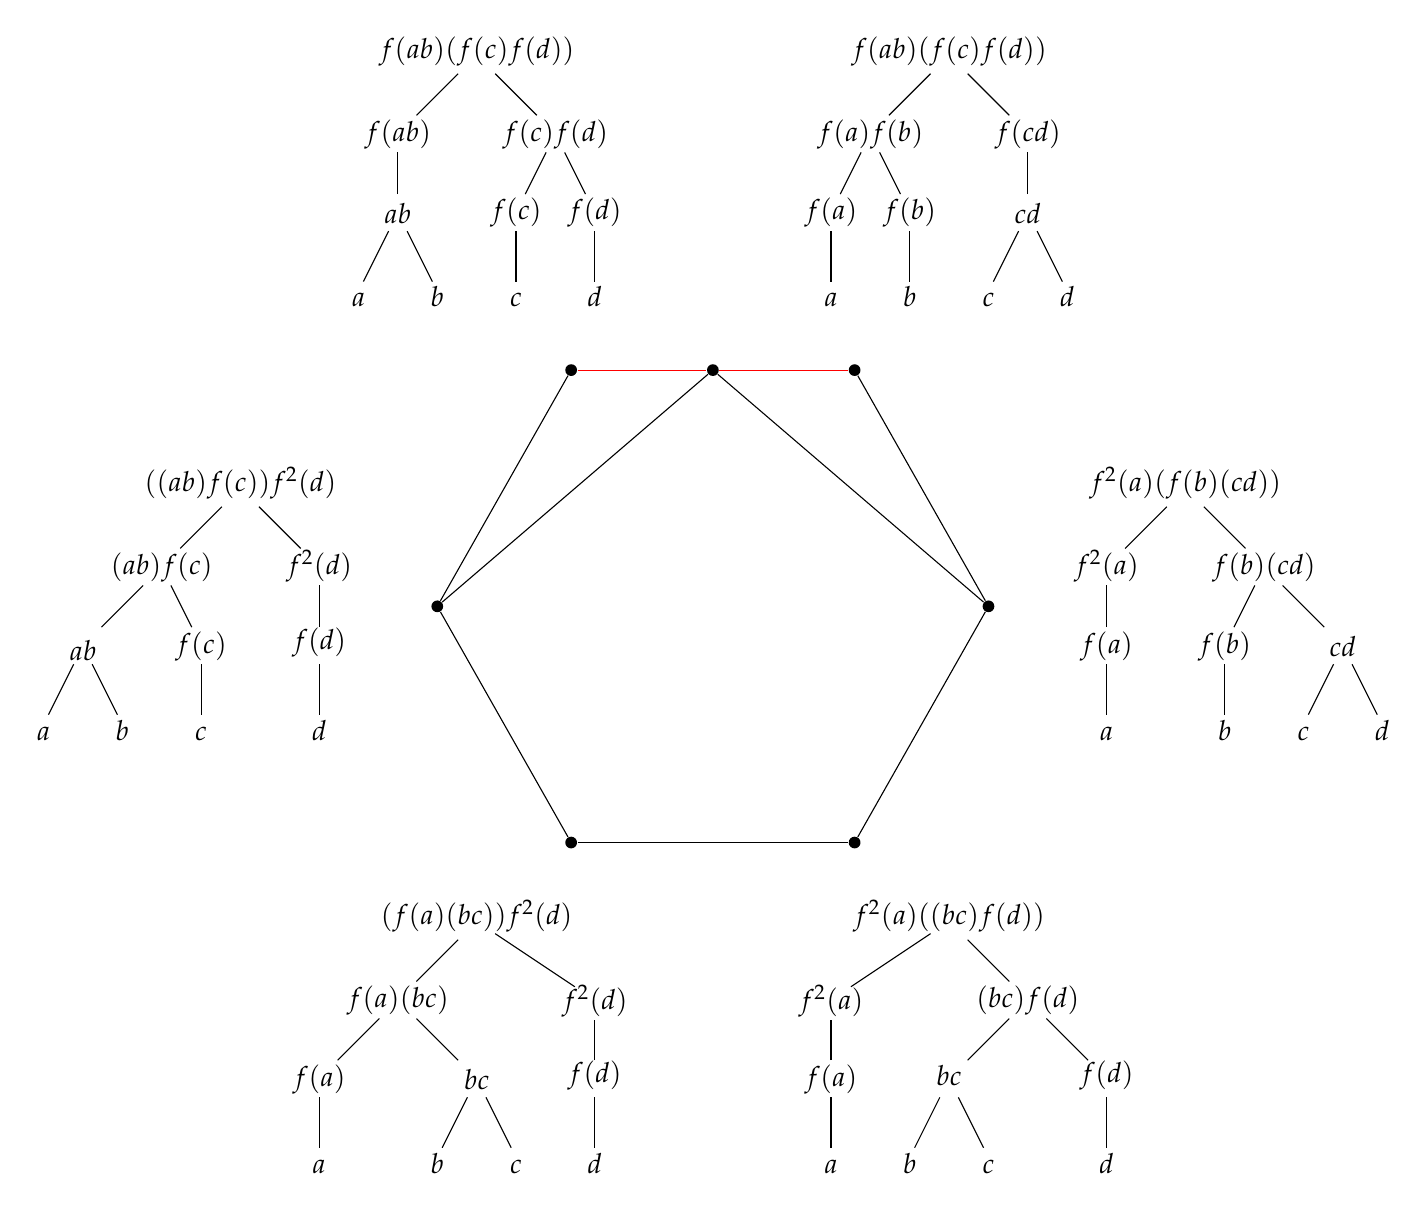
\begin{tikzpicture}
\node[label={[label distance=-0.45cm]90:$a$}] (a1) at (-0.5,0) {};
\node[label={[label distance=-0.45cm]90:$b$}] (a2) at (0.5,0) {};
\node[label={[label distance=-0.45cm]90:$c$}] (a3) at (1.5,0) {};
\node[label={[label distance=-0.45cm]90:$d$}] (a4) at (2.5,0) {};
\node[label={[label distance=-0.5cm]90:$ab$}, inner sep=6.5pt] (b1) at (0,1) {};
\node[label={[label distance=-0.55cm]90:$f(c)$}, inner sep=6.5pt] (b2) at (1.5,1) {};
\node[label={[label distance=-0.55cm]90:$f(d)$}, inner sep=6.5pt] (b3) at (2.5,1) {};
\node[label={[label distance=-0.55cm]90:$f(ab)$}, inner sep=6.5pt] (c1) at (0,2) {};
\node[label={[label distance=-0.55cm]90:$f(c)f(d)$}, inner sep=6.5pt] (c2) at (2,2) {};
\node[label={[label distance=-0.5cm]90:$f(ab)(f(c)f(d))$}, inner sep=6.5pt] (d1) at (1,3) {};
\draw (a1) -- (b1);
\draw (a2) -- (b1);
\draw (a3) -- (b2);
\draw (a4) -- (b3);
\draw (b1) -- (c1);
\draw (b2) -- (c2);
\draw (b3) -- (c2);
\draw (c1) -- (d1);
\draw (c2) -- (d1);

\node[label={[label distance=-0.45cm]90:$a$}] (aa1) at (5.5,0) {};
\node[label={[label distance=-0.45cm]90:$b$}] (aa2) at (6.5,0) {};
\node[label={[label distance=-0.45cm]90:$c$}] (aa3) at (7.5,0) {};
\node[label={[label distance=-0.45cm]90:$d$}] (aa4) at (8.5,0) {};
\node[label={[label distance=-0.5cm]90:$cd$}, inner sep=6.5pt] (bb1) at (8,1) {};
\node[label={[label distance=-0.55cm]90:$f(a)$}, inner sep=6.5pt] (bb2) at (5.5,1) {};
\node[label={[label distance=-0.55cm]90:$f(b)$}, inner sep=6.5pt] (bb3) at (6.5,1) {};
\node[label={[label distance=-0.55cm]90:$f(cd)$}, inner sep=6.5pt] (cc1) at (8,2) {};
\node[label={[label distance=-0.55cm]90:$f(a)f(b)$}, inner sep=6.5pt] (cc2) at (6,2) {};
\node[label={[label distance=-0.5cm]90:$f(ab)(f(c)f(d))$}, inner sep=6.5pt] (dd1) at (7,3) {};
\draw (aa1) -- (bb2);
\draw (aa2) -- (bb3);
\draw (aa3) -- (bb1);
\draw (aa4) -- (bb1);
\draw (bb1) -- (cc1);
\draw (bb2) -- (cc2);
\draw (bb3) -- (cc2);
\draw (cc1) -- (dd1);
\draw (cc2) -- (dd1);

\node[label={[label distance=-0.45cm]90:$a$}] (aaa1) at (9,-5.5) {};
\node[label={[label distance=-0.45cm]90:$b$}] (aaa2) at (10.5,-5.5) {};
\node[label={[label distance=-0.45cm]90:$c$}] (aaa3) at (11.5,-5.5) {};
\node[label={[label distance=-0.45cm]90:$d$}] (aaa4) at (12.5,-5.5) {};
\node[label={[label distance=-0.5cm]90:$cd$}, inner sep=6.5pt] (bbb1) at (12,-4.5) {};
\node[label={[label distance=-0.55cm]90:$f(a)$}, inner sep=6.5pt] (bbb2) at (9,-4.5) {};
\node[label={[label distance=-0.55cm]90:$f(b)$}, inner sep=6.5pt] (bbb3) at (10.5,-4.5) {};
\node[label={[label distance=-0.55cm]90:$f(b)(cd)$}, inner sep=6.5pt] (ccc1) at (11,-3.5) {};
\node[label={[label distance=-0.55cm]90:$f^2 (a)$}, inner sep=6.5pt] (ccc2) at (9,-3.5) {};
\node[label={[label distance=-0.5cm]90:$f^2 (a)(f(b)(cd))$}, inner sep=6.5pt] (ddd1) at (10,-2.5) {};
\draw (aaa1) -- (bbb2);
\draw (aaa2) -- (bbb3);
\draw (aaa3) -- (bbb1);
\draw (aaa4) -- (bbb1);
\draw (bbb1) -- (ccc1);
\draw (bbb2) -- (ccc2);
\draw (bbb3) -- (ccc1);
\draw (ccc1) -- (ddd1);
\draw (ccc2) -- (ddd1);

\node[label={[label distance=-0.45cm]90:$a$}] (aaaa1) at (5.5,-11) {};
\node[label={[label distance=-0.45cm]90:$b$}] (aaaa2) at (6.5,-11) {};
\node[label={[label distance=-0.45cm]90:$c$}] (aaaa3) at (7.5,-11) {};
\node[label={[label distance=-0.45cm]90:$d$}] (aaaa4) at (9,-11) {};
\node[label={[label distance=-0.5cm]90:$f(d)$}, inner sep=6.5pt] (bbbb1) at (9,-10) {};
\node[label={[label distance=-0.55cm]90:$f(a)$}, inner sep=6.5pt] (bbbb2) at (5.5,-10) {};
\node[label={[label distance=-0.45cm]90:$bc$}, inner sep=6.5pt] (bbbb3) at (7,-10) {};
\node[label={[label distance=-0.55cm]90:$(bc)f(d)$}, inner sep=6.5pt] (cccc1) at (8,-9) {};
\node[label={[label distance=-0.6cm]90:$f^2 (a)$}, inner sep=7pt] (cccc2) at (5.5,-9) {};
\node[label={[label distance=-0.5cm]90:$f^2 (a)((bc)f(d))$}, inner sep=6.5pt] (dddd1) at (7,-8) {};
\draw (aaaa1) -- (bbbb2);
\draw (aaaa2) -- (bbbb3);
\draw (aaaa3) -- (bbbb3);
\draw (aaaa4) -- (bbbb1);
\draw (bbbb1) -- (cccc1);
\draw (bbbb2) -- (cccc2);
\draw (bbbb3) -- (cccc1);
\draw (cccc1) -- (dddd1);
\draw (cccc2) -- (dddd1);

\node[label={[label distance=-0.45cm]90:$a$}] (aaaaa1) at (-1,-11) {};
\node[label={[label distance=-0.45cm]90:$b$}] (aaaaa2) at (0.5,-11) {};
\node[label={[label distance=-0.45cm]90:$c$}] (aaaaa3) at (1.5,-11) {};
\node[label={[label distance=-0.45cm]90:$d$}] (aaaaa4) at (2.5,-11) {};
\node[label={[label distance=-0.5cm]90:$f(d)$}, inner sep=6.5pt] (bbbbb1) at (2.5,-10) {};
\node[label={[label distance=-0.55cm]90:$f(a)$}, inner sep=6.5pt] (bbbbb2) at (-1,-10) {};
\node[label={[label distance=-0.5cm]90:$bc$}, inner sep=6.5pt] (bbbbb3) at (1,-10) {};
\node[label={[label distance=-0.6cm]90:$f^2 (d)$}, inner sep=7pt] (ccccc1) at (2.5,-9) {};
\node[label={[label distance=-0.55cm]90:$f(a)(bc)$}, inner sep=6.5pt] (ccccc2) at (0,-9) {};
\node[label={[label distance=-0.5cm]90:$(f(a)(bc))f^2 (d)$}, inner sep=6.5pt] (ddddd1) at (1,-8) {};
\draw (aaaaa1) -- (bbbbb2);
\draw (aaaaa2) -- (bbbbb3);
\draw (aaaaa3) -- (bbbbb3);
\draw (aaaaa4) -- (bbbbb1);
\draw (bbbbb1) -- (ccccc1);
\draw (bbbbb2) -- (ccccc2);
\draw (bbbbb3) -- (ccccc2);
\draw (ccccc1) -- (ddddd1);
\draw (ccccc2) -- (ddddd1);

\node[label={[label distance=-0.45cm]90:$a$}] (aaa1) at (-4.5,-5.5) {};
\node[label={[label distance=-0.45cm]90:$b$}] (aaa2) at (-3.5,-5.5) {};
\node[label={[label distance=-0.45cm]90:$c$}] (aaa3) at (-2.5,-5.5) {};
\node[label={[label distance=-0.45cm]90:$d$}] (aaa4) at (-1,-5.5) {};
\node[label={[label distance=-0.5cm]90:$f(d)$}, inner sep=6.5pt] (bbb1) at (-1,-4.5) {};
\node[label={[label distance=-0.55cm]90:$ab$}, inner sep=6.5pt] (bbb2) at (-4,-4.5) {};
\node[label={[label distance=-0.55cm]90:$f(c)$}, inner sep=6.5pt] (bbb3) at (-2.5,-4.5) {};
\node[label={[label distance=-0.55cm]90:$f^2 (d)$}, inner sep=6.5pt] (ccc1) at (-1,-3.5) {};
\node[label={[label distance=-0.55cm]90:$(ab)f(c)$}, inner sep=6.5pt] (ccc2) at (-3,-3.5) {};
\node[label={[label distance=-0.5cm]90:$((ab)f(c))f^2 (d)$}, inner sep=6.5pt] (ddd1) at (-2,-2.5) {};
\draw (aaa1) -- (bbb2);
\draw (aaa2) -- (bbb2);
\draw (aaa3) -- (bbb3);
\draw (aaa4) -- (bbb1);
\draw (bbb1) -- (ccc1);
\draw (bbb2) -- (ccc2);
\draw (bbb3) -- (ccc2);
\draw (ccc1) -- (ddd1);
\draw (ccc2) -- (ddd1);

\node[circle, fill=black, inner sep=1.5pt, label=below left:$$] (w1) at (2.2,-1) {$$};
\node[circle, fill=black, inner sep=1.5pt, label=below left:$$] (w2) at (5.8,-1) {$$};
\node[circle, fill=black, inner sep=1.5pt, label=below left:$$] (w3) at (7.5,-4) {$$};
\node[circle, fill=black, inner sep=1.5pt, label=below left:$$] (w4) at (5.8,-7) {$$};
\node[circle, fill=black, inner sep=1.5pt, label=below left:$$] (w5) at (2.2,-7) {$$};
\node[circle, fill=black, inner sep=1.5pt, label=below left:$$] (w6) at (0.5,-4) {$$};
\node[circle, fill=black, inner sep=1.5pt, label=below left:$$] (w7) at (4,-1) {$$};
\draw (w1)[color=red] -- (w7);
\draw[color=red] (w7) -- (w2);
\draw (w2) -- (w3);
\draw (w3) -- (w4);
\draw (w4) -- (w5);
\draw (w5) -- (w6);
\draw (w6) -- (w1);
\draw (w3) -- (w7);
\draw (w6) -- (w7);


\end{tikzpicture} \end{center}

\end{rem}

\begin{theorem} Let $(A,\mu,f)$ be a homassociative $R$-algebra
such that the $R$-algebra $(A,\mu)$ is unital with identity $e\in A$
and cancellative. Then we have
\[
f^{2}(a)=a.
\]

for all $a\in A$.

\end{theorem}

\begin{proof} Since $(A,\mu,f)$ is a homassociative $R$-algebra,
it follows from the homassociativity condition we have
\[
a\star f(b)=f(a)\star b=f(a\star b),
\]

for all $a,b\in A$. In particular, when $a=e$, we have $f(b)=f(e)\star b$.
Since $(A,\mu,f)$ is also a permutative $R$-algebra, it follows
from the permutativity law together with the homassociativity condition
that we have
\begin{align*}
f(a\star b)= & f(e)\star(f(a)\star f(b))=f(a)\star f^{2}(b)
\end{align*}

In particular, when $a=e$, we have $f^{2}(b)=f(e)\star f(b)$ for
all $b\in A$. Since $f(e)^{2}=e$ in any permutative $R$-algebra
with identity $e$, it then follows that we have 
\begin{align*}
f^{2}(b) & =f(e)\star f(b)\\
 & =f(e)\star(f(e)\star b)\\
 & =(f(e)\star f(e))\star b\\
 & =b
\end{align*}

\end{proof}

\section*{Idea}

If $A$ is not cancellative, then we have 
\[
f(f(a)f(b))=f(f(e)f(ab))
\]

This follows since 

Now
\[
f(a(bc))=f(1)(f(a)f(bc))=f(1)(f(a)bf(c))=f(1)(f(ab)f(c))=f((ab)c)
\]

Therefore if $f$ is injective, then $\cdot$ is associative. One
way we can create a permutative algebra from a hom-associative algebra
is by twisting it by a $3$-cocyle $\alpha$:
\[
(ab)f(c)=\alpha_{a,b,c}f(a)(bc)
\]

Then it follows

\begin{align*}
f(ab)(f(c)f(d)) & =\alpha_{ab,f(c),f(d)}^{-1}((ab)f(c))f^{2}(d)\\
 & =\alpha_{ab,f(c),f(d)}^{-1}\alpha_{a,b,c}(f(a)(bc))f^{2}(d)\\
 & =\alpha_{ab,f(c),f(d)}^{-1}\alpha_{a,b,c}\alpha_{f(a),bc,f(d)}f^{2}(a)((bc)f(d))\\
 & =\alpha_{ab,f(c),f(d)}^{-1}\alpha_{a,b,c}\alpha_{f(a),bc,f(d)}\alpha_{b,c,d}f^{2}(a)(f(b)(cd))\\
 & =\alpha_{ab,f(c),f(d)}^{-1}\alpha_{a,b,c}\alpha_{f(a),bc,f(d)}\alpha_{b,c,d}\alpha_{f(a),f(b),cd}^{-1}(f(a)f(b))f(cd).
\end{align*}

Now set $\beta_{a,b,c,d}=\alpha_{ab,f(c),f(d)}^{-1}\alpha_{a,b,c}\alpha_{f(a),bc,f(d)}\alpha_{b,c,d}\alpha_{f(a),f(b),cd}^{-1}$.
Then 
\[
f(ab)(f(c)f(d))=(f(ab)f(c))f(d)=
\]
\[
(d\beta)_{a,b,c,d,e}=\beta_{b,c,d,e}\beta_{ab,c,d,e}^{-1}\beta_{a,bc,d,e}\beta_{a,b,cd,e}^{-1}\beta_{a,b,c,de}\beta_{a,b,c,d}^{-1}
\]

This is 
\[
\beta_{b,c,d,e}=\alpha_{bc,f(d),f(e)}^{-1}\alpha_{b,c,d}\alpha_{f(b),cd,f(e)}\alpha_{c,d,e}\alpha_{f(b),f(c),de}^{-1}
\]
\[
\beta_{ab,c,d,e}^{-1}=\alpha_{abc,f(d),f(e)}\alpha_{ab,c,d}^{-1}\alpha_{f(ab),cd,f(e)}^{-1}\alpha_{c,d,e}^{-1}\alpha_{f(ab),f(c),de}
\]
\[
\beta_{a,bc,d,e}=\alpha_{abc,f(d),f(e)}^{-1}\alpha_{a,bc,d}\alpha_{f(a),bcd,f(e)}\alpha_{bc,d,e}\alpha_{f(a),f(bc),de}^{-1}
\]

\[
\beta_{a,b,cd,e}^{-1}=\alpha_{ab,f(cd),f(e)}\alpha_{a,b,cd}^{-1}\alpha_{f(a),bcd,f(e)}^{-1}\alpha_{b,cd,e}^{-1}\alpha_{f(a),f(b),cde}
\]

\[
\beta_{a,b,c,de}=\alpha_{ab,f(c),f(de)}^{-1}\alpha_{a,b,c}\alpha_{f(a),bc,f(de)}\alpha_{b,c,de}\alpha_{f(a),f(b),cde}^{-1}
\]

\[
\beta_{a,b,c,d}^{-1}=\alpha_{ab,f(c),f(d)}\alpha_{a,b,c}^{-1}\alpha_{f(a),bc,f(d)}^{-1}\alpha_{b,c,d}^{-1}\alpha_{f(a),f(b),cd}
\]

So 
\[
(d\beta)_{a,b,c,d,e}=\alpha_{a,b,c}^{-1}\alpha_{c,d,e}\alpha_{abc,f(d),f(e)}\alpha_{f(a),bcd,f(e)}\alpha_{f(a),f(b),cde}
\]

\section*{Are The Octonions Permutative?}

The \textbf{octonions} $\mathbb{O}$ are a normed division algebra
over the real numbers. They are not commutative nor associative, but
satisfy a weaker form of associativity, namely they are alternative.
This means for all $x,y\in\mathbb{O}$, we have 
\[
x(xy)=(xx)y\quad\mbox{and}\quad(yx)x=y(xx)
\]

Thus if they were to be $f$-associative for some $f:\mathbb{O}\to\mathbb{O}$,
we must have 
\[
f(x)(xf^{-1}(y))=x(xy)
\]

So if $f(x)=x$ for any $x\in\mathbb{O}$, then $f(x)=x$ for all
$x\in\mathbb{O}$. 

\subsection*{New Section}

Formula $a\star b=f^{-1}(f(e)\star f(a)\star f(b))$. 
\[
a\star b=-(-a\star-b)
\]

Quaternions
\begin{center}
\begin{tabular}{c|c|c|c|c}
$\star$ & $1$ & $i$ & $j$ & $k$\tabularnewline
\hline 
$1$ & $1$ & $i$ & $j$ & $k$\tabularnewline
\hline 
$i$ & $i$ & $-1$ & $k$ & $-j$\tabularnewline
\hline 
$j$ & $j$ & $-k$ & $-1$ & $i$\tabularnewline
\hline 
$k=ij$ & $k$ & $j$ & $-i$ & $-1$\tabularnewline
\end{tabular}
\par\end{center}

$(\mathbb{Z}_{4},\star)$
\begin{center}
\begin{tabular}{c|c|c|c|c}
$\star$ & $0$ & $1$ & $2$ & $3$\tabularnewline
\hline 
$0$ & $0$ & $1$ & $2$ & $3$\tabularnewline
\hline 
$1$ & $1$ & $a$ & $b$ & $c$\tabularnewline
\hline 
$2$ & $2$ & $d$ & $e$ & $-d$\tabularnewline
\hline 
$3$ & $3$ & $-c$ & $-b$ & $-a$\tabularnewline
\end{tabular}
\par\end{center}

$1\star2=-\left(3\star2\right)$

$2\star2=-\left(2\star2\right)$

$1\star3=-\left(3\star1\right)$

$2\star1=-\left(2\star3\right)$

$1\star1=-\left(3\star3\right)$

Now assume $(a\star b)\star c=-a\star(b\star-c)$

$1\star3=(1\star0)\star3=3\star(0\star1)=3\star1$

$2\star3=(2\star0)\star3=2\star(0\star1)=2\star1$

$1\star2=(1\star0)\star2=3\star(0\star2)=3\star2$

$1\star1=(1\star0)\star1=3\star(0\star3)=3\star3$

$a\star b=(a\star0)\star b=f(a)\star(0\star f^{-1}(b))=f(a)\star f^{-1}(b)$.
So if $f(a)=b$, then $a\star b=b\star a$.

$(a\star b)\star c=f(a)\star(b\star f^{-1}(c))$. So if $f(a)=c$,
then $(a\star b)\star c=c\star(b\star a)$.

$a\star b=f^{-1}(f(a)\star f(b))$. 

$a\star1=(1\star1)\star1=3\star(1\star3)=3\star c$

$b\star3=(1\star2)\star3=3\star(2\star1)=3\star d$
\begin{center}
\begin{tabular}{c|c|c|c|c}
$\star$ & $0$ & $1$ & $2$ & $3$\tabularnewline
\hline 
$0$ & $0$ & $1$ & $2$ & $3$\tabularnewline
\hline 
$1$ & $1$ & $a$ & $b$ & $c$\tabularnewline
\hline 
$2$ & $2$ & $b$ & $e$ & $b$\tabularnewline
\hline 
$3$ & $3$ & $c$ & $b$ & $a$\tabularnewline
\end{tabular}
\par\end{center}

Next
\begin{center}
\begin{tabular}{c|c|c|c|c|c|c|c|c}
 & $0$ & $1$ & $2$ & $3$ & $4$ & $5$ & $6$ & $7$\tabularnewline
\hline 
$0$ & $0$ & $1$ & $2$ & $3$ & $4$ & $5$ & $6$ & $7$\tabularnewline
\hline 
$1$ & $1$ & $a$ & $b$ & $c$ & $d$ & $e$ & $f$ & $g$\tabularnewline
\hline 
$2$ & $2$ & $h$ & $i$ & $j$ & $k$ & $l$ & $m$ & $n$\tabularnewline
\hline 
$3$ & $3$ & $o$ & $p$ & $q$ & $r$ & $s$ & $t$ & $u$\tabularnewline
\hline 
$4$ & $4$ & $v$ & $w$ & $x$ & $y$ & $-x$ & $-w$ & $-v$\tabularnewline
\hline 
$5$ & $5$ & $-u$ & $-t$ & $-s$ & $-r$ & $-q$ & $-p$ & $-o$\tabularnewline
\hline 
$6$ & $6$ & $-n$ & $-m$ & $-l$ & $-k$ & $-j$ & $-i$ & $-h$\tabularnewline
\hline 
$7$ & $7$ & $-g$ & $-f$ & $-e$ & $-d$ & $-c$ & $-b$ & $-a$\tabularnewline
\end{tabular}
\par\end{center}

Now assume $(a\star b)\star c=-a\star(b\star-c)$

$1\star7=7\star1$
\begin{center}
\begin{tabular}{c|c|c|c|c|c|c|c|c}
 & $0$ & $1$ & $2$ & $3$ & $4$ & $5$ & $6$ & $7$\tabularnewline
\hline 
$0$ & $0$ & $1$ & $2$ & $3$ & $4$ & $5$ & $6$ & $7$\tabularnewline
\hline 
$1$ & $1$ & $a$ & $b$ & $c$ & $d$ & $e$ & $f$ & $g$\tabularnewline
\hline 
$2$ & $2$ & $h$ & $i$ & $j$ & $k$ & $l$ & $m$ & $n$\tabularnewline
\hline 
$3$ & $3$ & $o$ & $p$ & $q$ & $r$ & $s$ & $t$ & $u$\tabularnewline
\hline 
$4$ & $4$ & $v$ & $w$ & $x$ & $y$ & $x$ & $w$ & $v$\tabularnewline
\hline 
$5$ & $5$ & $u$ & $t$ & $s$ & $r$ & $q$ & $p$ & $o$\tabularnewline
\hline 
$6$ & $6$ & $n$ & $m$ & $l$ & $k$ & $j$ & $i$ & $h$\tabularnewline
\hline 
$7$ & $7$ & $g$ & $f$ & $e$ & $d$ & $c$ & $b$ & $a$\tabularnewline
\end{tabular}
\par\end{center}

$ $

Or $a\star b=3\star(3a\star3b)$
\begin{center}
\begin{tabular}{c|c|c|c|c|c|c|c|c}
 & $0$ & $1$ & $2$ & $3$ & $4$ & $5$ & $6$ & $7$\tabularnewline
\hline 
$0$ & $0$ & $1$ & $2$ & $3$ & $4$ & $5$ & $6$ & $7$\tabularnewline
\hline 
$1$ & $1$ & $a$ & $b$ & $c$ & $d$ & $e$ & $f$ & $g$\tabularnewline
\hline 
$2$ & $2$ & $h$ & $i$ & $j$ & $k$ & $l$ & $m$ & $n$\tabularnewline
\hline 
$3$ & $3$ & $3c$ & $3f$ & $3a$ & $3d$ & $3g$ & $3b$ & $3e$\tabularnewline
\hline 
$4$ & $4$ & $v$ & $w$ & $3v$ & $\{0,4\}$ & $x$ & $3w$ & $3x$\tabularnewline
\hline 
$5$ & $5$ & $o$ & $p$ & $q$ & $r$ & $s$ & $t$ & $u$\tabularnewline
\hline 
$6$ & $6$ & $3l$ & $3j$ & $3h$ & $3m$ & $3k$ & $3i$ & $3n$\tabularnewline
\hline 
$7$ & $7$ & $3q$ & $3t$ & $3o$ & $3r$ & $3u$ & $3p$ & $3s$\tabularnewline
\end{tabular}
\par\end{center}

Now assume $a\star b=(a\star0)\star b=3a\star3b$
\begin{center}
\begin{tabular}{c|c|c|c|c|c|c|c|c|c}
$(t_{4})_{g,h}$ & $e$ & $(12)$ & $(23)$ & $(34)$ & $(123)$ & $(12)(34)$ & $(13)(24)$ & $(14)(23)$ & $...$\tabularnewline
\hline 
$e$ & $1$ & $1$ & $1$ & $1$ & $1$ & $1$ & $1$ & $1$ & \tabularnewline
\hline 
$(12)$ & $1$ & $1$ & $1$ & $1$ & $1$ &  &  &  & \tabularnewline
\hline 
$(23)$ & $1$ & $1$ & $1$ & $1$ & $1$ &  &  &  & \tabularnewline
\hline 
$(34)$ & $1$ & $-1$ & $1$ & $1$ & $1$ &  &  &  & \tabularnewline
\hline 
$(12)(34)$ & $1$ & $-1$ & $-1$ & $1$ & $1$ & $-1$ & $1$ & $1$ & \tabularnewline
\hline 
$(13)(24)$ & $1$ &  &  &  &  & $-1$ & $-1$ & $1$ & \tabularnewline
\hline 
$(14)(23)$ & $1$ &  &  &  &  & $1$ & $-1$ & $-1$ & \tabularnewline
\hline 
$...$ &  &  &  &  &  &  &  &  & \tabularnewline
\end{tabular}
\par\end{center}

\section*{References}

https://arxiv.org/pdf/1504.03019.pdf
\end{document}
